\exercisesetinstructions{, find the fluid force exerted on the given plate, submerged in water with a weight density of 62.4 lb/ft$^3$.}

\exercise{\begin{minipage}{\linewidth}
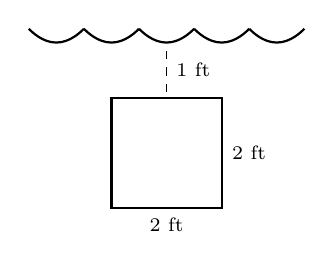
\begin{tikzpicture}[xscale=.7,yscale=.7]			
\draw [shift={(-1,0)},thick] (0,0) -- node [below,pos=.5] {\scriptsize 2 ft} (2,0)-- node [right,pos=.5] {\scriptsize 2 ft} (2,2) -- (0,2) -- cycle;
\foreach \x in {-2,-1,0,1,2}{%
		\begin{scope}[shift={(\x*1,3)}]		
		\draw [thick] (-.5,.25) parabola bend (0,0) (.5,.25);
		\end{scope}
}
\draw [dashed] (0,2.1) -- node [right,pos=.5] {\scriptsize 1 ft} (0,2.9);
\end{tikzpicture}
\end{minipage}}{499.2 lb}

\exercise{\begin{minipage}{\linewidth}
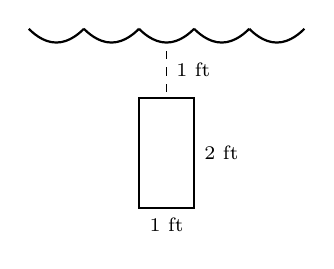
\begin{tikzpicture}[xscale=.7,yscale=.7]			
\draw [shift={(-.5,0)},thick] (0,0) -- node [below,pos=.5] {\scriptsize 1 ft} (1,0)-- node [right,pos=.5] {\scriptsize 2 ft} (1,2) -- (0,2) -- cycle;
\foreach \x in {-2,-1,0,1,2}{%
		\begin{scope}[shift={(\x*1,3)}]		
		\draw [thick] (-.5,.25) parabola bend (0,0) (.5,.25);
		\end{scope}
}
\draw [dashed] (0,2.1) -- node [right,pos=.5] {\scriptsize 1 ft} (0,2.9);
\end{tikzpicture}
\end{minipage}}{249.6 lb}

\exercise{\begin{minipage}{\linewidth}
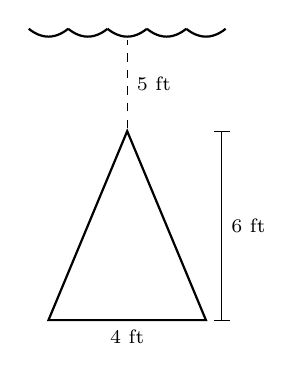
\begin{tikzpicture}[xscale=.5,yscale=.4]			
\draw [thick] (0,0) -- (-2,-6) -- node [below,pos=.5] {\scriptsize 4 ft} (2,-6) -- cycle;
\foreach \x in {-2,-1,0,1,2}{%
		\begin{scope}[shift={(\x*1,3)}]		
		\draw [thick] (-.5,.25) parabola bend (0,0) (.5,.25);
		\end{scope}
}
\draw [dashed] (0,0.1) -- node [right,pos=.5] {\scriptsize 5 ft} (0,2.9);
\draw (2.2,-6) -- (2.6,-6)
			(2.2,0) -- (2.6,0)
			(2.4,-6) -- node [pos=.5,right] {\scriptsize 6 ft} (2.4,0);			
\end{tikzpicture}
\end{minipage}}{6739.2 lb}

\exercise{\begin{minipage}{\linewidth}
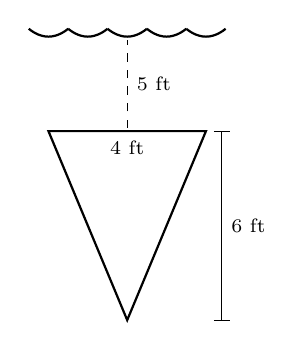
\begin{tikzpicture}[xscale=.5,yscale=.4]			
\draw [thick] (0,0) -- (-2,6) -- node [below,pos=.5] {\scriptsize 4 ft} (2,6) -- cycle;
\foreach \x in {-2,-1,0,1,2}{%
		\begin{scope}[shift={(\x*1,9)}]		
		\draw [thick] (-.5,.25) parabola bend (0,0) (.5,.25);
		\end{scope}
}
\draw [dashed] (0,6.1) -- node [right,pos=.5] {\scriptsize 5 ft} (0,8.9);
\draw (2.2,6) -- (2.6,6)
			(2.2,0) -- (2.6,0)
			(2.4,6) -- node [pos=.5,right] {\scriptsize 6 ft} (2.4,0);			
\end{tikzpicture}
\end{minipage}}{5241.6 lb}

\exercise{\begin{minipage}{\linewidth}
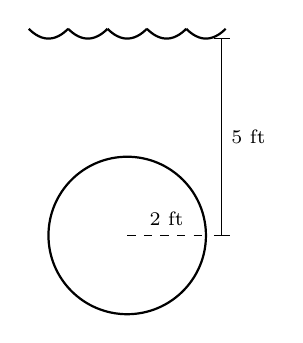
\begin{tikzpicture}[xscale=.5,yscale=.5]			
\draw [thick] (0,0) circle (2);
\foreach \x in {-2,-1,0,1,2}{%
		\begin{scope}[shift={(\x*1,5)}]		
		\draw [thick] (-.5,.25) parabola bend (0,0) (.5,.25);
		\end{scope}
}
\draw [dashed] (0,0) -- node [above,pos=.5] {\scriptsize 2 ft} (2,0);
\draw (2.2,5) -- (2.6,5)
			(2.2,0) -- (2.6,0)
			(2.4,5) -- node [pos=.5,right] {\scriptsize 5 ft} (2.4,0);			
\end{tikzpicture}
\end{minipage}}{3920.7 lb}

\exercise{\begin{minipage}{\linewidth}
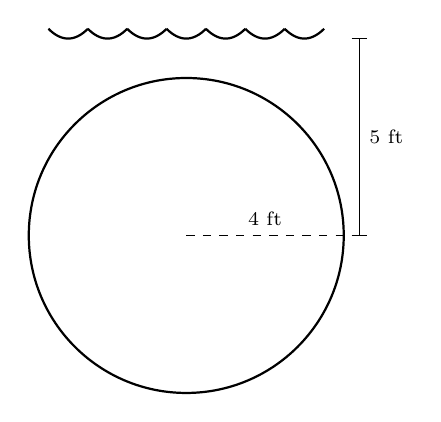
\begin{tikzpicture}[xscale=.5,yscale=.5]			
\draw [thick] (0,0) circle (4);
\foreach \x in {-3,-2,-1,0,1,2,3}{%
		\begin{scope}[shift={(\x*1,5)}]		
		\draw [thick] (-.5,.25) parabola bend (0,0) (.5,.25);
		\end{scope}
}
\draw [dashed] (0,0) -- node [above,pos=.5] {\scriptsize 4 ft} (4,0);
\draw (4.2,5) -- (4.6,5)
			(4.2,0) -- (4.6,0)
			(4.4,5) -- node [pos=.5,right] {\scriptsize 5 ft} (4.4,0);			
\end{tikzpicture}
\end{minipage}}{15682.8 lb}

\exercise{\begin{minipage}{\linewidth}
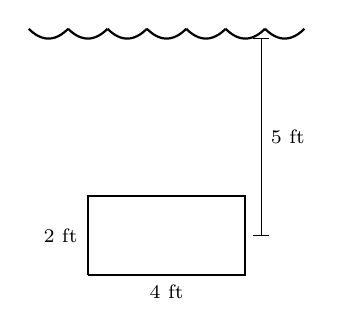
\begin{tikzpicture}[xscale=.5,yscale=.5]			
\draw [thick] (-2,-1) -- node [below,pos=.5] {\scriptsize 4 ft} (2,-1) -- (2,1) -- (-2,1) -- node [left,pos=.5] {\scriptsize 2 ft} (-2,-1);
\foreach \x in {-3,-2,-1,0,1,2,3}{%
		\begin{scope}[shift={(\x*1,5)}]		
		\draw [thick] (-.5,.25) parabola bend (0,0) (.5,.25);
		\end{scope}
}
\draw (2.2,5) -- (2.6,5)
			(2.2,0) -- (2.6,0)
			(2.4,5) -- node [pos=.5,right] {\scriptsize 5 ft} (2.4,0);			
\end{tikzpicture}
\end{minipage}}{2496 lb}

\exercise{\begin{minipage}{\linewidth}
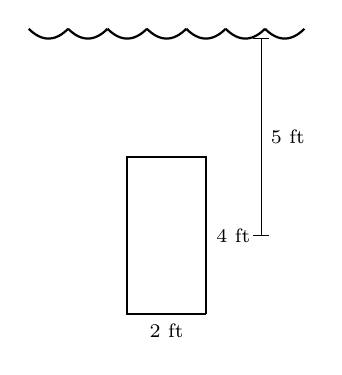
\begin{tikzpicture}[xscale=.5,yscale=.5]			
\draw [thick,rotate=90] (-2,-1) -- node [right,pos=.5] {\scriptsize 4 ft} (2,-1) -- (2,1) -- (-2,1) -- node [below,pos=.5] {\scriptsize 2 ft} (-2,-1);
\foreach \x in {-3,-2,-1,0,1,2,3}{%
		\begin{scope}[shift={(\x*1,5)}]		
		\draw [thick] (-.5,.25) parabola bend (0,0) (.5,.25);
		\end{scope}
}
\draw (2.2,5) -- (2.6,5)
			(2.2,0) -- (2.6,0)
			(2.4,5) -- node [pos=.5,right] {\scriptsize 5 ft} (2.4,0);			
\end{tikzpicture}
\end{minipage}}{2496 lb}

\exercise{\begin{minipage}{\linewidth}
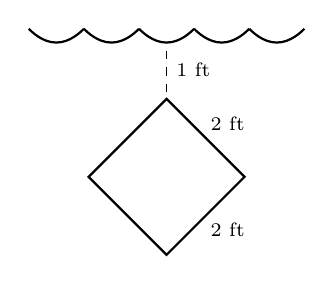
\begin{tikzpicture}[xscale=.7,yscale=.7]			
\draw [shift={(0,-.85)},thick,rotate=45] (0,0) -- node [shift={(8pt,-5pt)},pos=.5] {\scriptsize 2 ft} (2,0)-- node [shift={(8pt,5pt)},pos=.5] {\scriptsize 2 ft} (2,2) -- (0,2) -- cycle;
\foreach \x in {-2,-1,0,1,2}{%
		\begin{scope}[shift={(\x*1,3)}]		
		\draw [thick] (-.5,.25) parabola bend (0,0) (.5,.25);
		\end{scope}
}
\draw [dashed] (0,2.1) -- node [right,pos=.5] {\scriptsize 1 ft} (0,2.9);
\end{tikzpicture}
\end{minipage}}{602.59 lb}

\exercise{\begin{minipage}{\linewidth}
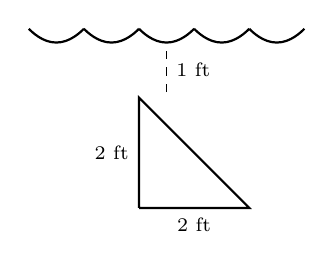
\begin{tikzpicture}[xscale=.7,yscale=.7]			
\draw [shift={(-.5,0)},thick] (0,0) -- node [below,pos=.5] {\scriptsize 2 ft} (2,0)--   (0,2) -- node [left,pos=.5] {\scriptsize 2 ft} (0,0);
\foreach \x in {-2,-1,0,1,2}{%
		\begin{scope}[shift={(\x*1,3)}]		
		\draw [thick] (-.5,.25) parabola bend (0,0) (.5,.25);
		\end{scope}
}
\draw [dashed] (0,2.1) -- node [right,pos=.5] {\scriptsize 1 ft} (0,2.9);
\end{tikzpicture}
\end{minipage}}{291.2 lb}

\exercisesetend
